\documentclass[9pt]{article}
% Libraries
\usepackage{titlesec} 
\usepackage{xcolor}
\usepackage{amsmath}
\usepackage{colortbl}
\usepackage[left=2.5cm,right=2.5cm,top=2.5cm,bottom=2cm]{geometry}
\usepackage{fancyhdr}
\usepackage{subfigure}
\usepackage{layouts}
\usepackage{graphicx}
\usepackage[yyyymmdd,hhmmss]{datetime}
\usepackage{hyperref}
\usepackage{helvet}

%------------------Color Set--------------------------
\definecolor{LightBlue}{RGB}{66, 163, 251}
\definecolor{DarkBlue}{RGB}{36, 100, 176}
\definecolor{LightGray}{gray}{.94}
\definecolor{DarkGray}{gray}{.172}
\definecolor{Orange}{RGB}{229, 133, 3}
\definecolor{MediumBlue}{RGB}{38, 119, 193}

%------------------Section Default Setting-------------
\titleformat*{\section}{\color{DarkBlue}\normalfont\bfseries\Huge}
\titleformat*{\subsection}{\color{LightBlue}\normalfont\bfseries\LARGE}
\titleformat*{\subsubsection}{\color{MediumBlue}\normalfont\bfseries\LARGE}

%-------------------Section Numbers Removal------------
\setcounter{secnumdepth}{0}

%-------------------Set New Default Font------------
\renewcommand\familydefault{\sfdefault}

%-------------------------Header & Footer------------------------
\pagestyle{fancy}
\fancyhf{}
\renewcommand{\footrulewidth}{0.4pt}

% Header
\fancyhead[L]{\ifthenelse{\value{page}=1}{ }{pyHRV Report}}
\fancyhead[R]{\ifthenelse{\value{page}=1}{ }{\subject, \gender, \age, \today\, \currenttime}}

% Footer
\lfoot{HRV results \& report generated with pyHRV (v.\version)\\\url{https://github.com/PGomes92/pyhrv}}
\rfoot{\thepage\ of \pageref{page:lastpage}}

%-------------------------Custom Table Functions------------------------
\newcolumntype{L}[1]{>{\raggedright\let\newline\\\arraybackslash\hspace{0pt}}m{#1}}
\newcolumntype{C}[1]{>{\centering\let\newline\\\arraybackslash\hspace{0pt}}m{#1}}
\newcolumntype{R}[1]{>{\raggedleft\let\newline\\\arraybackslash\hspace{0pt}}m{#1}}

\newcommand{\btcell}[1]{{\cellcolor{LightBlue}\textbf{#1}}}
\newcommand{\bcell}[1]{{\cellcolor{LightBlue}{#1}}}
\newcommand{\gcell}[1]{{\cellcolor{LightGray}{#1}}}

\newcommand{\dline}{\hline\hline}

%-------------------------Define new boolean variables to toggle section visibility------------------------
\newif\ifecgsignal
\newif\iftachogram
\newif\ifhistogram
\newif\ifhrheatplot
\newif\iftdomain
\newif\ifwelch
\newif\ifar
\newif\iflomb
\newif\iffdomain
\newif\ifndomain
\newif\ifpoincare
\newif\ifdfa
\newif\ifsampen
\input{parameters.tex}

%------------------Document----------------------------
\begin{document}

%-------------------------Content------------------------
    % pyHRV Logo
    \begin{center}
        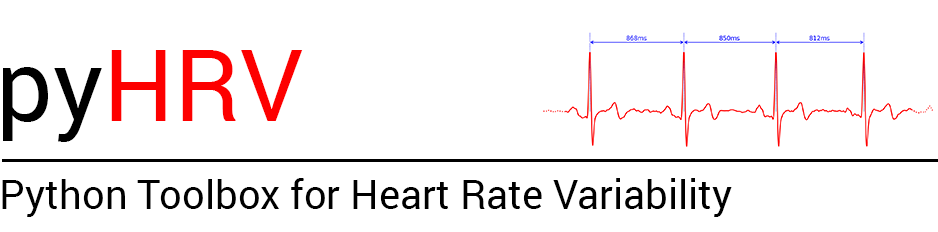
\includegraphics[width=\textwidth]{pyhrv.png}
    \end{center}
    
    % Report
    \section{Report}

    % General Info Table
    \subsection{General Information}
\begin{table}[h]
    % Metadata
    \begin{tabular}{L{4cm}L{12cm}}
         \hline
         \bcell{Experiment}    & \gcell{\experiment}                \\
         \bcell{Subject}       & \gcell{\subject}                   \\
         \bcell{Gender, Age}   & \gcell{\gender\ , \age}              \\
         \bcell{Date}          & \gcell{\today\ , \currenttime}      \\
         \bcell{Comment}       & \gcell{\comment}                   \\
         \hline
    \end{tabular}
\end{table}

    % Add ECG Signal
    \ifecgsignal
        test
        \begin{center}
            \includegraphics[width=\textwidth]{figures/ecgplot.png}
            \vspace{-5mm}
        \end{center}
        \vspace{-5mm}
    \fi

    % Add tachogram plot
    \iftachogram
        \begin{center}
            \includegraphics[width=\textwidth]{figures/tachogram.png}
        \end{center}
    \vspace{-5mm}
    \fi

    % Add HR heatplot
    \ifhrheatplot
        \begin{center}
            \includegraphics[width=\textwidth]{figures/hrheatplot.png}
        \end{center}
        \vspace{-5mm}
    \fi

    % Add Time Domain Results
    \iftdomain \newpage
\subsection{Time Domain Results}
    \begin{table}[h!]
        \begin{tabular}{*{2}{L{3cm}C{3cm}C{1cm}}}
            % Basic NNI Parameters
            % --------------------------------------------------------------------------------------
            \hline
            \rowcolor{LightBlue}
            \textbf{Parameter}                      & \textbf{Value}    & \textbf{Unit} &
            \textbf{Parameter}                      & \textbf{Value}    & \textbf{Unit} \\\hline
            % --------------------------------------------------------------------------------------
            \multicolumn{6}{l}{\gcell{}\textbf{NNI Parameters}}                                 \\
            \gcell{NNI}                             & \nnicounter       & -             &
            \gcell{}$\overline{\text{NNI}}$         & \nnimean          & ms            \\
            \gcell{}\text{$NNI_{min}$}              & \nnimin           & ms            &
            \gcell{}\text{$NNI_{max}$}              & \nnimax           & ms            \\
            \gcell{}SDNN                            & \sdnn             & ms            & 
            \gcell{}RMSSD                           & \rmssd            & ms            \\
            \gcell{}SDANN                           & \sdann            & ms            &
            \gcell{}\text{$SDNN_{index}$}           & \sdnnindex        & ms            \\
            \gcell{}NN20                            & \nntwenty         & -             &
            \gcell{}pNN20                           & \pnntwenty        & -             \\
            \gcell{}NN50                            & \nnfifty          & -             &
            \gcell{}pNN50                           & \pnnfifty         & -             \\
            \hline
            % Delta NNI
            % --------------------------------------------------------------------------------------
            \multicolumn{6}{l}{\gcell{}\textbf{NNI Differences Parameters}}             \\
            \gcell{}\text{$\overline{\Delta NNI}$}       & \nnidiffmean      & ms            &
            \gcell{}\text{$\Delta NNI_{min}$}            & \nnidiffmin       & ms            \\
            \gcell{}\text{$\Delta NNI_{max}$}            & \nnidiffmax       & ms            &
            \gcell{}SDSD                                 & \sdsd             & ms       \\\hline
            % HR Parameters
            % --------------------------------------------------------------------------------------
            \multicolumn{6}{l}{\gcell{}\textbf{HR Parameters}}                          \\
            \gcell{}\text{$\overline{HR}$}          & \hrmean           & bpm           &
            \gcell{}\text{$HR_{min}$}               & \hrmin            & bpm           \\
            \gcell{}\text{$HR_{max}$}               & \hrmax            & bpm           &
            \gcell{}\text{$\sigma(HR)$}                  & \hrstd            & bpm           \\\hline
            % HR Parameters
            % --------------------------------------------------------------------------------------
            \multicolumn{6}{l}{\gcell{}\textbf{Geometrical Parameters}}                 \\
            \gcell{}Triangular Index                & \triindex         & ms            &
            \gcell{}TINN                            & n/a$^1$ & -            \\\hline
            \multicolumn{6}{l}{}
        \end{tabular}
    \end{table}
    \vspace{-5mm}
    \footnotesize{$^1$TINN function is not working properly in the current pyHRV version and computes incorrect results, reason for which it is not shown in this report}
    \begin{figure}[h!]
        \includegraphics[width=\textwidth]{figures/histogram.png}
        \caption{Histogram of the NNI series.}
    \end{figure}
    \vfill \fi
    
    % Add Frequency Domain Results
    \iffdomain \newpage
\newcommand{\cwidth}{2.1cm}
\subsection{Frequency Domain Parameters}

\ifwelch % FFT Based Welchs Method
\begin{table}[h!]
	\begin{tabular}{L{3.5cm}C{\cwidth}C{\cwidth}C{\cwidth}C{\cwidth}C{\cwidth}C{\cwidth}}
		\hline\hline
		\multicolumn{6}{c}{\textbf{Welch's Method}}\\
	    \hline\hline
		\rowcolor{LightBlue}        & Unit      & ULF           & VLF         &  LF          & HF               	\\
		\hline
		\gcell{Peak Frequencies}    & $Hz$      & \fftulfpeak	 & \fftvlfpeak   & \fftlfpeak    & \ffthfpeak    	\\
		\gcell{Absolute Powers}     & $ms^2$    & \fftulfabs    & \fftvlfabs    & \fftlfabs     & \ffthfabs     	\\
		\gcell{Relative Powers}     & $\%$      & \fftulfrel    & \fftvlfrel    & \fftlfrel     & \ffthfrel     	\\
		\gcell{Logarithmic Powers}  & $-$       & \fftulflog    & \fftvlflog    & \fftlflog     & \ffthflog     	\\
		\gcell{Relative Powers}     & $-$       & -             & -             & \fftlfrel     & \ffthfrel     	\\
		\gcell{LF/HF Ratio}         & $-$       & \multicolumn{4}{c}{\fftratio}                             		\\
		\gcell{Total Power}         & $ms^2$    & \multicolumn{4}{c}{\ffttotal}                            		\\\hline
	\end{tabular}
\end{table}
\vspace{-2mm}
\begin{table}[h!]
	\footnotesize
	\begin{tabular}{L{3.5cm}L{4cm}L{1.5cm}L{4cm}L{1.5cm}}
		\textbf{Configuration:}										&
		Resampling frequency: 		&	\fftresamplingfrequency Hz	&
		Window:						&	\fftwindow					\\ &
		Interpolation:				&	\fftinterpolation			&
		NFFT (over entire signal):	&	\fftnfft 					\\
	\end{tabular}
\end{table}
 \fi
\ifar % Autoregressive Method
\begin{table}[h!]
	\centering
	\begin{tabular}{L{3.5cm}C{\cwidth}C{\cwidth}C{\cwidth}C{\cwidth}C{\cwidth}C{\cwidth}}
		\hline\hline
		\multicolumn{6}{c}{\textbf{Autoregressive Method}}\\
	    \hline\hline
		\rowcolor{LightBlue}        & Unit      & ULF          & VLF          &  LF          & HF               \\
		\hline
		\gcell{Peak Frequencies}    & $Hz$      & \arulfpeak	& \arvlfpeak   & \arlfpeak    & \arhfpeak  \\
		\gcell{Absolute Powers}     & $ms^2$    & \arulfabs   	& \arvlfabs    & \arlfabs     & \arhfabs   \\
		\gcell{Relative Powers}     & $\%$      & \arulfrel   	& \arvlfrel    & \arlfrel     & \arhfrel   \\
		\gcell{Logarithmic Powers}  & $-$       & \arulflog   	& \arvlflog    & \arlflog     & \arhflog   \\
		\gcell{Relative Powers}     & $-$       & -           	& -            & \arlfrel     & \arhfrel   \\
		\gcell{LF/HF Ratio}         & $-$       & \multicolumn{4}{c}{\arratio}                            \\
		\gcell{Total Power}         & $ms^2$    & \multicolumn{4}{c}{\artotal}                            \\\hline
	\end{tabular}
\end{table}
\vspace{-2mm}
\begin{table}[h!]
	\footnotesize
	\begin{tabular}{L{3.5cm}L{4cm}L{1.5cm}L{4cm}L{1.5cm}}
		\textbf{Configuration:}						&
		Model Order: 				&	\arorder 	&
		NFFT (over entire signal):	&	\arnfft		\\
	\end{tabular}
\end{table}
 \fi
\iflomb % Lomb-Scargle Method
\begin{table}[h!]
	\centering
	\begin{tabular}{L{3.5cm}C{\cwidth}C{\cwidth}C{\cwidth}C{\cwidth}C{\cwidth}C{\cwidth}}
		\hline\hline
		\multicolumn{6}{c}{\textbf{Lomb-Scargle Method}}\\
	    \hline\hline
		\rowcolor{LightBlue}        & Unit      & ULF           	& VLF         	&  LF          	  & HF              \\
		\hline
		\gcell{Peak Frequencies}    & $Hz$      & \lombulfpeak	 	& \lombvlfpeak  & \lomblfpeak    & \lombhfpeak     \\
		\gcell{Absolute Powers}     & $ms^2$    & \lombulfabs    	& \lombvlfabs   & \lomblfabs     & \lombhfabs      \\
		\gcell{Relative Powers}     & $\%$      & \lombulfrel    	& \lombvlfrel   & \lomblfrel     & \lombhfrel      \\
		\gcell{Logarithmic Powers}  & $-$       & \lombulflog    	& \lombvlflog   & \lomblflog     & \lombhflog      \\
		\gcell{Relative Powers}     & $-$       & -             	& -             & \lomblfrel     & \lombhfrel      \\
		\gcell{LF/HF Ratio}         & $-$       & \multicolumn{4}{c}{\lombratio}                             			\\
		\gcell{Total Power}         & $ms^2$    & \multicolumn{4}{c}{\lombtotal}                            			\\\hline
	\end{tabular}
\end{table}
\vspace{-2mm}
\begin{table}[h!]
	\footnotesize
	\begin{tabular}{L{3.5cm}L{4cm}L{1.5cm}L{4cm}L{1.5cm}}
		\textbf{Configuration:}									&
		Moving Average Window Size:	 &	\lombma					&
		NFFT (over entire signal):	 &	\lombnfft 				\\
	\end{tabular}
\end{table}
 \fi

\begin{table*}[h!]
	\centering
	\begin{tabular}{L{3.5cm}C{\cwidth}C{\cwidth}C{\cwidth}C{\cwidth}C{\cwidth}C{\cwidth}}
	    \hline\hline
		\multicolumn{6}{c}{\textbf{Selected Frequency Bands}}					\\
		\hline\hline
		\gcell{ULF Band}	& $Hz$	& \multicolumn{4}{c}{\ulflow\  - \ulfhigh} 	\\
		\gcell{VLF Band}   	& $Hz$  & \multicolumn{4}{c}{\vlflow\  - \vlfhigh}  \\
		\gcell{LF Band}		& $Hz$  & \multicolumn{4}{c}{\lflow\  - \lfhigh}	\\
		\gcell{HF Band}    	& $Hz$  & \multicolumn{4}{c}{\hflow\  - \hfhigh}	\\\hline
	\end{tabular}
\end{table*}

\newpage
\begin{figure}[t!]
	\centering
	% Welch PSD
	\ifwelch
		\includegraphics[width=\textwidth]{figures/fftplot.png}
		\vspace{-7mm}
		\caption{Welch's method with resampling frequency of \fftresamplingfrequency\ Hz, \fftwindow\ window, \fftinterpolation\ interpolation, and \fftnfft\ samples over the entire signal.}
		\vfill
	\fi
    % AR PSD
    \ifar
		\includegraphics[width=\textwidth]{figures/arplot.png}
		\vspace{-7mm}
		\caption{Autoregressive method with model order \arorder\ and \arnfft\ samples over the entire signal.}
		\vfill
	\fi
    % Lomb PSD
    \iflomb
		\includegraphics[width=\textwidth]{figures/lombplot.png}
		\vspace{-7mm}
		\caption{Lomb-Scargle method with moving average window size of \lombma\ samples and \lombnfft\ samples over the entire signal.}
		\vfill
	\fi
\end{figure}
\vfill
\clearpage
 \fi

    % Add Nonlinear Parameters
    \ifndomain  \newpage
\subsection{Nonlinear Parameters}

% Table
\begin{table}[h!]
    \begin{tabular}{*{2}{L{3cm}C{2cm}C{2cm}}}
        \hline\rowcolor{LightBlue}
        \btcell{Parameter}                  & \btcell{Value}    & \btcell{Unit}     &
        \btcell{Parameter}                  & \btcell{Value}    & \btcell{Unit}      \\\hline
    \end{tabular}
    % Poincare Results
    \ifpoincare
        \begin{tabular}{*{2}{L{3cm}C{3cm}C{1cm}}}
                \multicolumn{6}{l}{\gcell{\textbf{Poincar\'e Plot Parameters}}}     \\
                \gcell{SD1}                 & \sdone            & ms                &
                \gcell{SD2}                 & \sdone            & ms                \\
                \gcell{SD1/SD2}             & \sdratio          & ms                &
                \gcell{Ellipse Area S}      & \ellipsearea      & ms                \\\hline
        \end{tabular}
    \fi
    % DFA
    \ifdfa
        \begin{tabular}{*{2}{L{3cm}C{3cm}C{1cm}}}
            \multicolumn{6}{l}{\gcell{\textbf{Detrended Fluctuation Analysis}}}     \\
            \gcell{${\alpha}_1$}            & \dfaalphaone      & -                 &
            \gcell{${\alpha}_2$}            & \dfaalphatwo      & -                 \\\hline
        \end{tabular}
    \fi
    % Sample Entropy Results
    \ifsampen
        \begin{tabular}{*{2}{L{3cm}C{3cm}C{1cm}}}
            \multicolumn{6}{l}{\gcell{\textbf{Sample Entropy}}}                     \\
            \gcell{Sample Entropy}          & \sampen           & -                 &
            \gcell{-}                       & -                 & ms                \\\hline
        \end{tabular}
    \fi
\end{table}

% Poincare Plot
\ifpoincare
    \begin{minipage}{.475\textwidth}
        \centering
        \includegraphics[width=\linewidth]{figures/poincareplot.png}
    \end{minipage}%
    \hfill
\fi
% DFA Plot
\ifdfa
    \begin{minipage}{.457\textwidth}
        \centering
        \includegraphics[width=\linewidth]{figures/dfaplot.png}
    \end{minipage}
\else
    \hfill
\fi

\vfill \fi

    % Add Glossary
    %%
%% Author: Pedro Gomes
%% 08/05/2019
%%
\textbf{Glossary}
\begin{table}[h!]
    \footnotesize
    \centering
    \begin{tabular}{L{2cm}L{15cm}}
            AR                      &   Autoregressive                                                              \\
            BPM                     &   Beats per Minute                                                            \\
            DFA                     &   Detrended Fluctuation Analysis                                              \\
            HF                      &   High Frequency Band                                                           \\
            HR                      &   Hear Rate                                                                     \\
            LF                      &   Low Frequency Band                                                            \\
            \text{$\Delta NNI$}     &   Differences between successive NNI                                            \\
            NNI                     &   Normal-to-Normal Intervals                                                    \\
            NNx                     &   \# of \text{$\Delta NNI$} > x ms                                              \\
            pNNx                    &   NNx / \# of NNI                                                               \\
            PSD                     &   Power Spectral Density                                                      \\
            RMSSD                   &   Root Mean of Squared \text{$\Delta NNI$}                                      \\
            SDANN                   &   Standard Deviation of the Mean of NNI in all 5 minute Segments                \\
            SDNN                    &   Standard Deviation of NNI                                                     \\
            \text{$SDNN_{index}$}   &   Standard Deviation of the Mean of NN Intervals in all 5 minut Segments      \\
            SDSD                    &   Standard Deviation of \text{$\Delta NNI$}                                     \\
            TINN                    &   Triangular Interpolation of the NNI Histogram                                 \\
            ULF                     &   Ultra Low Frequency Band                                                      \\
            VLF                     &   Very Low Frequency Band
    \end{tabular}
    \label{table:glossary}
\end{table}

    %-------------------------Content------------------------
    \label{page:lastpage}
\end{document}
